\chapter{Abordagem}
\label{sec:abordagem}

Este capítulo tem como principal objectivo descrever a metologia adoptada e ainda apresentar o planeamento do projecto tal como os desvios relativamente ao mesmo. Por fim será apresentada uma analise dos riscos associados ao projecto que poderão tem um impacto negativo no plano de desenvolvimento. Este conjunto de passos foca-se em atingir um produto final bem estruturado e funcional, utilando boas práticas de desenvolvimento de software


\section{Metodologia}
\label{metodologia}

A metodologia de desenvolvimento do projecto adoptada foi uma metodologia fortemente baseada em SCRUM\cite{scrum}, que será descrita (i. e. os aspectos mais importantes) nesta secção. Esta é a metodologia utilizada pela 10.digital e tendo em conta que esta metodologia ágil se encaixa perfeitamente nas necessidades do projecto, estes foram os factores decisivos para a escolha da mesma. 

Líder em desenvolvilmento àgil, o SCRUM, é uma metodologia apontada para projectos com foco em trazer valor ao cliente de forma incremental, através de iterações de curta duração, chamadas Sprints. Esta metodologia possibilita também a abordagem de problemas complexos de forma produtiva, prioritorizar tarefas durante a fase de desenvolvimento e ainda facilita a inclusão de novas funcionalidades sempre que ncessário. Desta forma o SCRUM proporciona uma gestão flexível do projecto e permite realizar pequenas alterações no planeamento, sem necessidade de interromper o desenvolvimento.

\subsection{Intervenientes}

Um aspecto determinante para o sucesso do SCRUM é o trabalho em equipa. Tipicamente nesta metodologia existem três papeis pré-definidos: \textit{Product Owner}, \textit{Scrum Master} e \textit{Scrum Team}.

O \textbf{\textit{Product Owner}} representa o cliente e é responsável por transmitir a visão do produto, ou por outras palavras, é responsável por maximizar o valor do produto e o trabalho da equipa de desenvolvimento (i. e. \textit{Scrum Master}). É responsável por organizar e priorizar as taferas no \textit{product backlog}.

O \textbf{\textit{Scrum Master}} tem um papel fundamental no desempenho da \textit{Scrum Team}. É responsável por garantir o cumprimento das práticas do SCRUM, ajudar e orintar a \textit{Scrum Team} especialmente nas dificuldades que vão surgindo ao longo do projedcto e, de forma gradual (i. e. respeitando as \textit{Sprints}), apresentar o trabalho realizado ao \textit{Product Owner}.

A \textbf{\textit{Scrum Team}} representa os elementos que constituem a equipa de desenvolvimento que com a orientação do \textit{Scrum Master}, monitorizam o trabalho que vai sendo feito e assim conseguir cumprir com as \textit{sprints backlog}. A \textit{Scrum Team} deve ser autónomae organizada.

\subsection{Processo}

O Desenvolviemento começa assim que o \textit{product backlog} estiver concluído e detalhado pelo \textit{Product Owner}. O \textit{product backlog} representa a lista requisitos necessários para atingir o produto final. 

Depois de definido o \textit{product backlog}, o \textit{Scrum Master}, juntamente com a \textit{Scrum Team} reunem e definem o tempo para cada \textit{Sprint}. Tipicamente as \textit{Sprints} tem duração entre 1 a 4 semanas e no final das mesmas é apresentado o trabalho realizado pela \textit{Scrum Team}. No inicio de cada \textit{Sprint} é criada a \textit{Sprint Backlog}. Na \textit{Sprint Backlog} é estipulado o conjunto de funcionalidades/tarefas a realizar durante a \textit{Sprint}. Na 10.digital a variável da velocidade não é implementada na \textit{Sprint Backlog}.

No inicio de cada dia é realizada a \textit{Daily Scrum}, uma reunião que tem uma duração de 15$\pm$5 minutos, onde, de forma informal, são discutidas as tarefas que devem ser implementadas nesse dia, o ponto de situação do projeto relativo ao dia anterior e caso haja algum impasse ou dificuldade na realização de alguma tarefa, imediatamente após a reunião (i. e. assim que possível) tentasse arranjar uma solução para o mesmo. 

No final de cada \textit{Sprint} há uma reunião (\textit{Sprint Review}) para verificar as tarefas que foram realizadas. Durante a reunião a \textit{Scrum Team} apresenta as novas funcionalidades implementadas para os restantes participantes que podem ser \textit{Product Owner}, \textit{Scrum Master}, clientes e outros colegas de trabalho. 

A Figura \ref{fig:scrum} sumariza todo o processo descrito anteriormente.



\begin{figure}[ht!]
	\begin{center}
		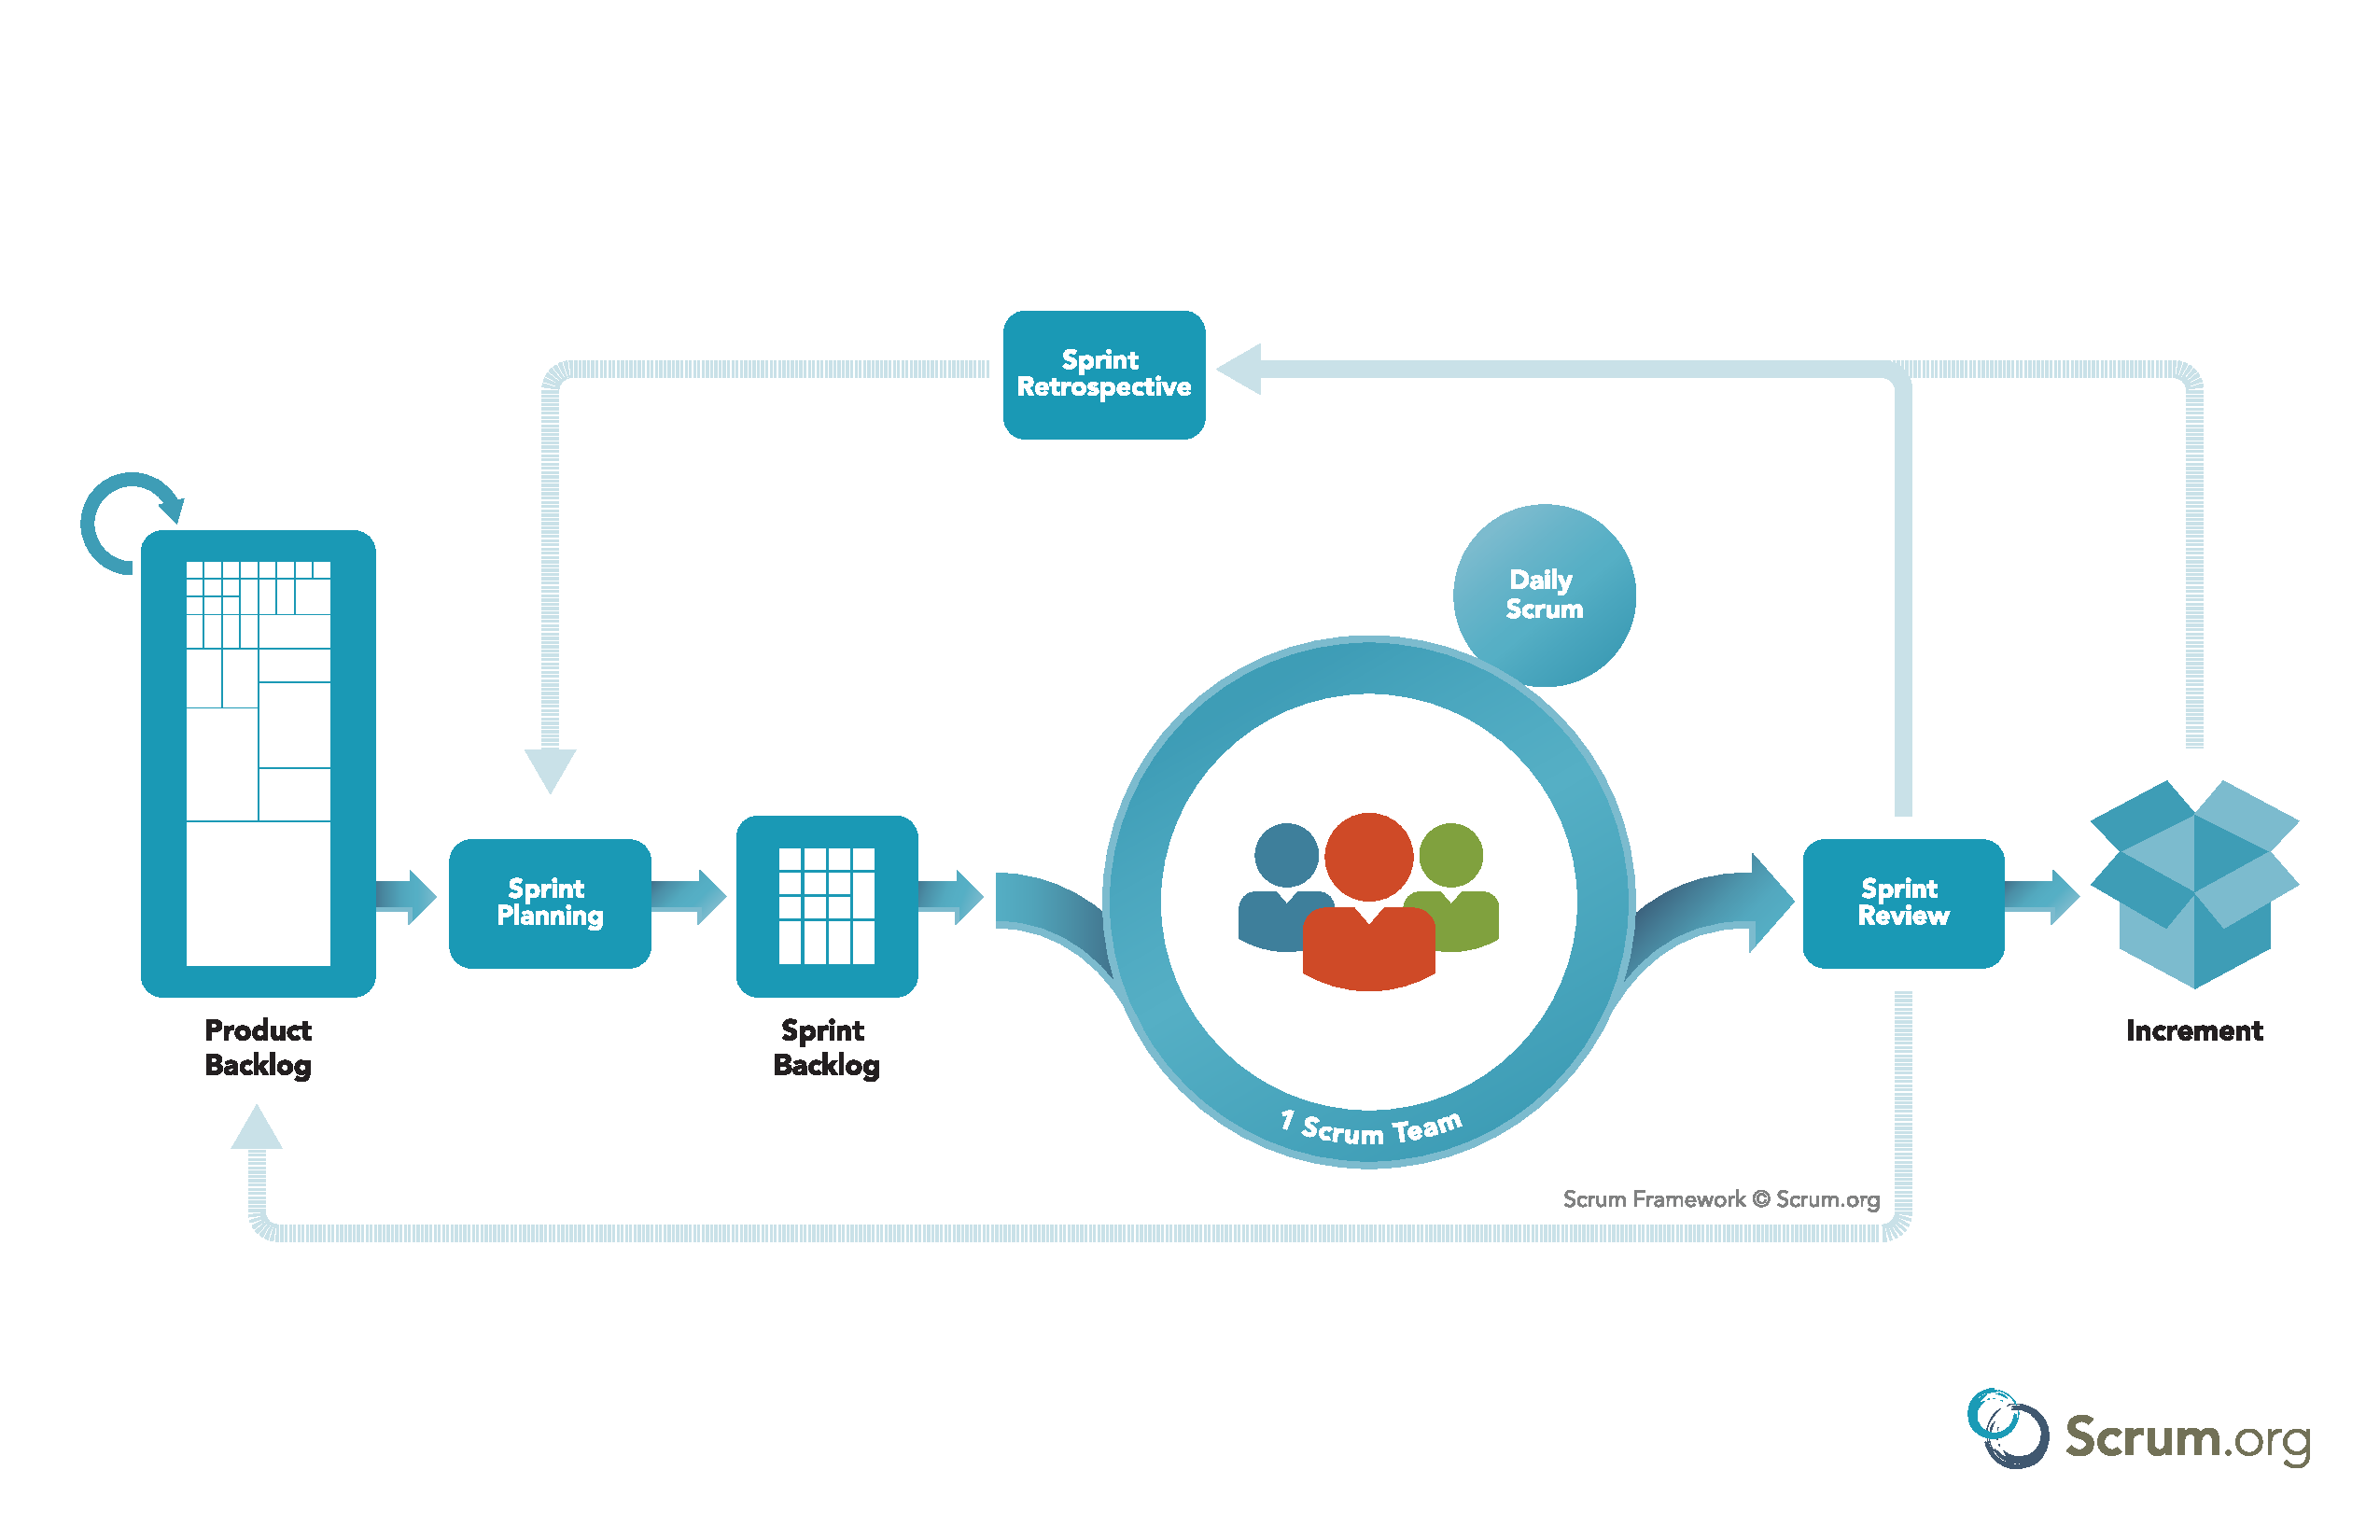
\includegraphics[width=1\textwidth]{img/scrum.pdf}
		\caption{Scrum Framework\cite{scrumimg}}
		\label{fig:scrum}
	\end{center}
\end{figure}

\newpage

\section{Planeamento}
\label{planeamento}

\begin{figure}[ht!]
	\begin{center}
		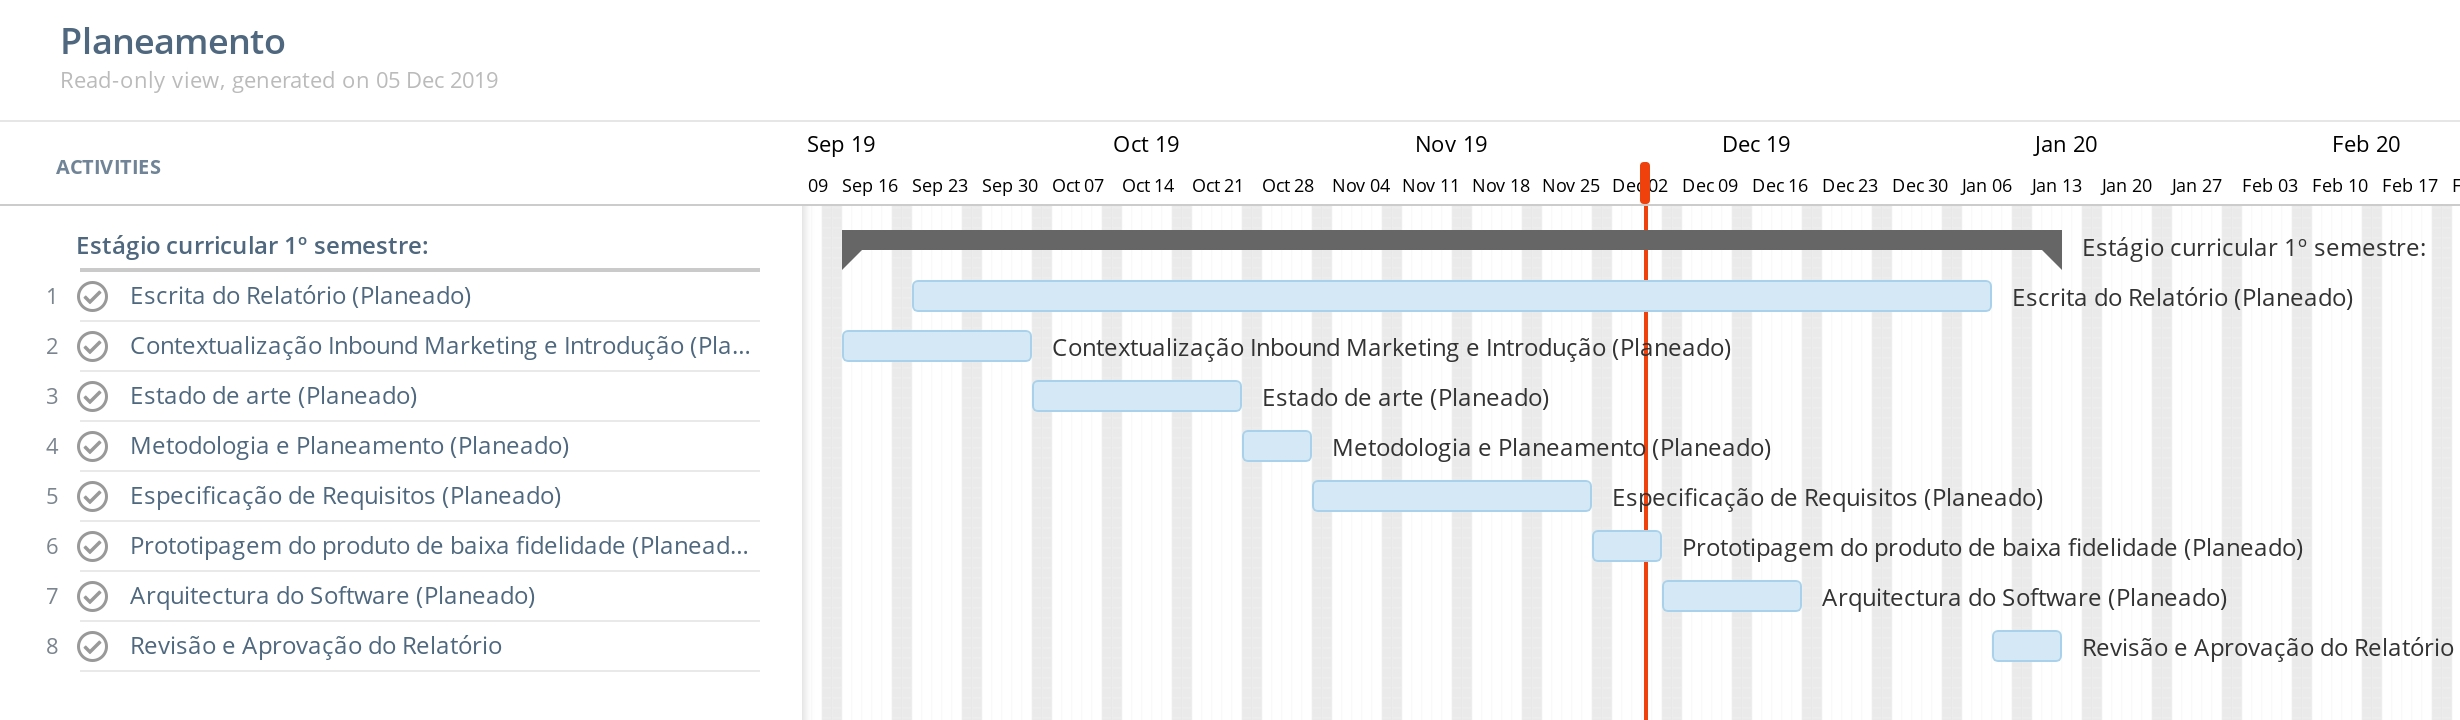
\includegraphics[width=1\textwidth]{img/gantt/semestre1.jpeg}
		\caption{Diagrama de Gantt - Planeamento do 1º semestre}
		\label{fig:gantt1}
	\end{center}
\end{figure}

\begin{figure}[ht!]
	\begin{center}
		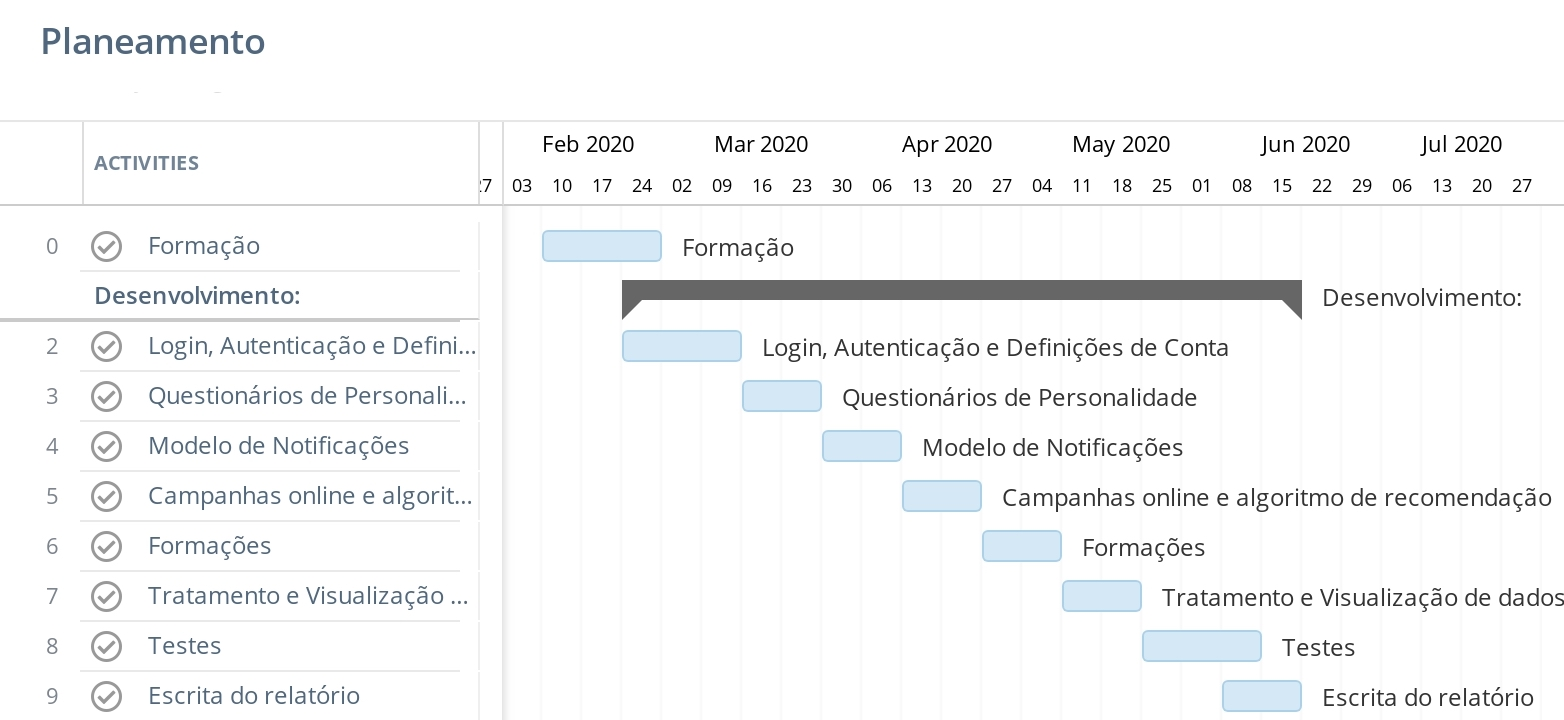
\includegraphics[width=1\textwidth]{img/gantt/semestre2.jpeg}
		\caption{Diagrama de Gantt - Planeamento do 2º semestre}
		\label{fig:gantt2}
	\end{center}
\end{figure}


\section{Ferramentas Utilizadas}
\label{ferramentas}


\section{Analise se Riscos}
\label{analiseriscos}
%-------------------------------------------------------------------------------------------------
\blankpage
%-------------------------------------------------------------------------------------------------

\glsresetall



